\chapter{Características de estructura del protón}\label{ch-ProtonStructureCh}

El protón, al ser considerado compuesto por quarks y gluones independientes entre sí, puede separar sus contribuciones energéticas por cada una de las partes. El \acrshort{bm} describe a los quarks como siendo confinados dentro del hadrón. Aunque hay varias versiones del modelo de bolsa, la característica principal es la fenomenología de confinamiento de quarks. Los gluones son bosones mediadores que transfieren las interacciones entre quarks. Como ya hemos detallado en la sección \ref{sec-PresTsa}, la energía y el número total de partículas para un sistema de quarks y gluones sin masa dentro de un hadrón están dadas por

\begin{equation}
N ={N}_{Q} + {N}_{G}  = \frac{16 \zeta(3)}{{\pi}^{2}}V{T}^{3}
\end{equation}

\begin{equation}
E = {E}_{Q} + {E}_{G} = \frac{37}{30} {\pi}^{2} V{T}^{4}.
\end{equation}

%\section*{Temperatura como función de la distacia al centro del protón}

\begin{wrapfigure}{r}{0.5\textwidth}
\centering
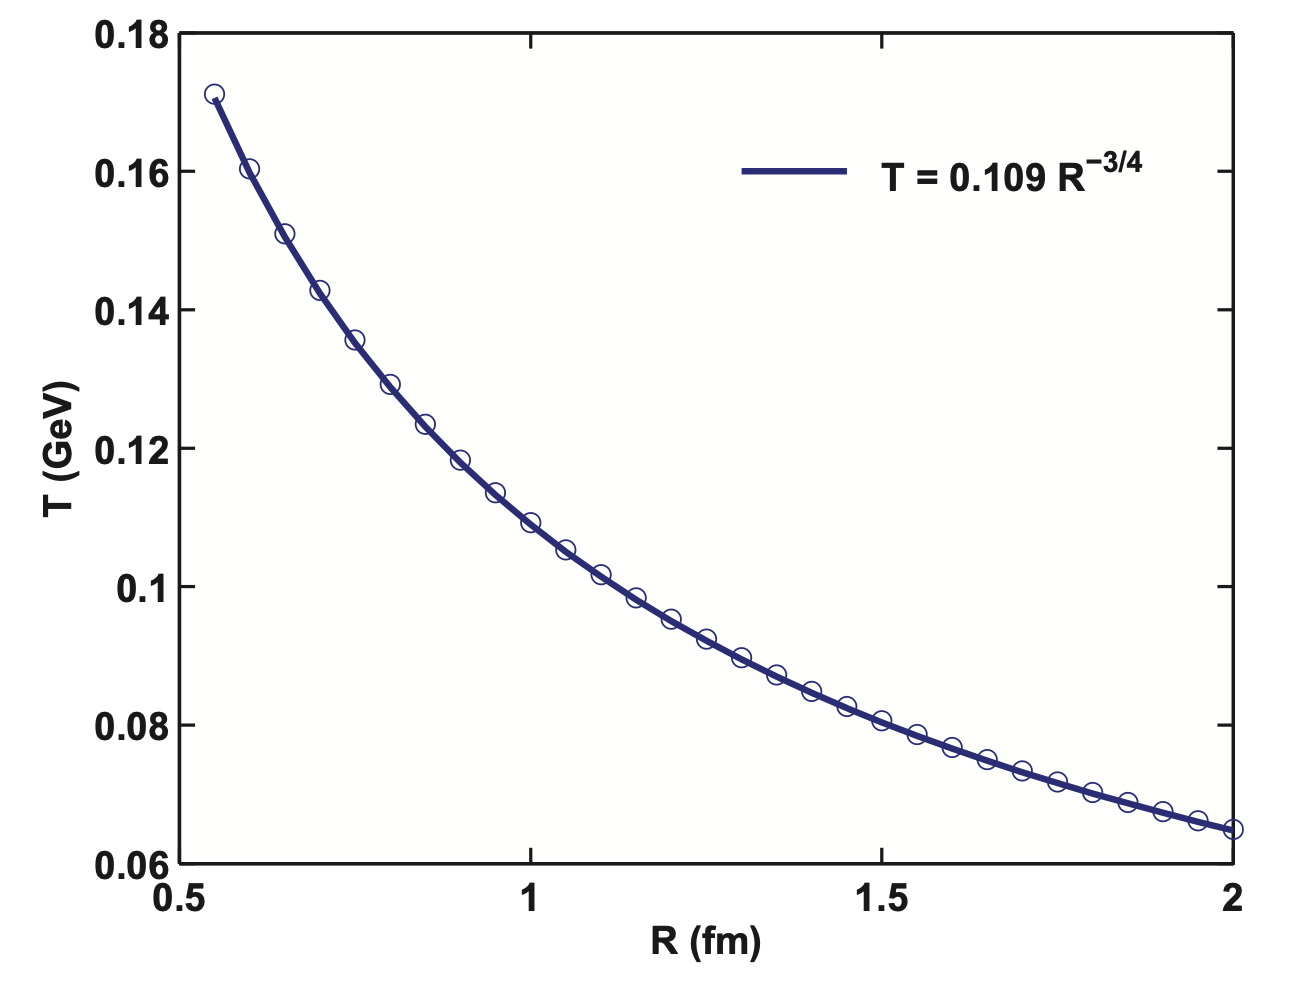
\includegraphics[width=0.5\textwidth]{./Images/T(R).png}
\caption[Temperatura como función del radio del protón]{\emph{Ajuste realizado a una simulación numérica de la temperatura dentro del protón como función del radio}}
\label{fig: T(r)}
\end{wrapfigure}

Tomando la masa de un nucleón como la energía total ${E}_{t} = M$, y siendo este como un sistema local en equilibrio térmico y despreciando el potencial químico, podemos calcular los cambios de temperatura con el radio del protón. De acuerdo con [Some characteristic parameters], se tiene una fórmula simulada numéricamente para la temperatura en función de la distacia al centro del protón, $r$, como 

\begin{equation}\label{eq-T(r)}
T = 0.109\left[ \frac{GeV}{fm}\right] {r}^{-3/4}, \quad (r  \text{ en fm})
\end{equation}

A alrededor de $1 \, \mathrm{fm}$, la temperatura es alrededor de $105 \, \mathrm{MeV}$. Cuando el radio de un protón es menor de $0.6 \, \mathrm{fm}$, la temperatura probablemente será aproximada a $170 \, \mathrm{MeV}$, cercana a la temperatura crítica a la que el hadron se rompe a quarks.

\begin{wrapfigure}{r}{0.4\textwidth}
\centering
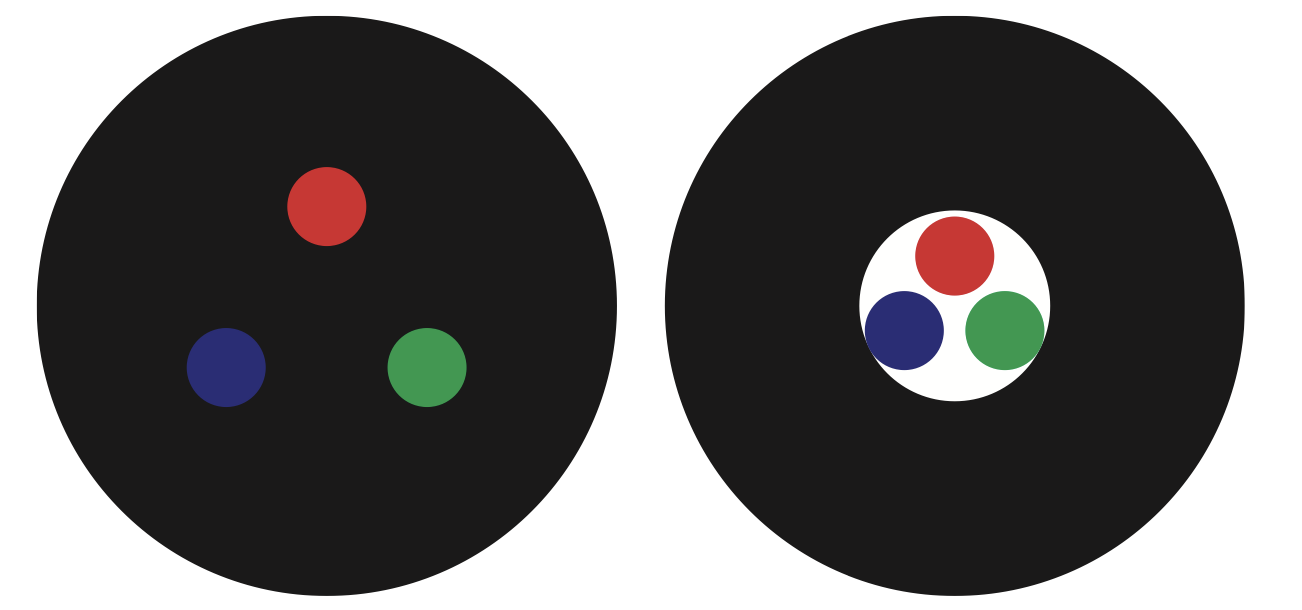
\includegraphics[width=0.4\textwidth]{./Images/Bag model-two scenaries.png}
\caption[Posibles estructuras del modelo de bolsa]{\emph{Tenemos dos posibilidades, i) que los quarks estén inmersos en un mar de gluones (izquierda) o ii) que los quarks estén \textbf{rodeados} por un mar de gluones(derecha)}}
\label{fig: 2Bag-models}
\end{wrapfigure}

%\section*{Presión de bolsa como función de la distancia al centro del protón}

Como vimos antes, en el capítulo \ref{ch-BagModel}, las soluciones a la ecuación \eqref{eq-condeigenval}, nos dan los límites de los radios de los hadrones considerando la relación ${\omega}_{n\kappa} = {p}_{n\kappa}{R}$, tenemos que para el estado más bajo accesible del sistema (que notaremos como ${\omega}_{1 \, -1} = {\omega}_{0} = 2.04$) y así para un protón, tenemos que la máxima energía cinética accesible para los quarks y gluones en el interior está dado por

\begin{equation}\label{eq-maxp}
{{p}_{0}}_{m} = \frac{2.04}{R}
\end{equation}

Si tomamos ${{p}_{0}}_{m}$ como el límite superior, podemos separar la energía de quarks del total de un protón

\begin{equation}
{E}_{Q} = \frac{\left({g}_{Q} + {g}_{\bar{Q}} \right) V}{2{\pi}^{2}{\hbar}^{3}} \int_{0}^{{{p}_{0}}_{m}} \frac{{p}^{3} \mathrm{d}p}{1 + {e}^{p/T(r)}}
\end{equation}

Por simplicidad, despreciamos el potencial químico, $\mu=0$, tratamos los quarks como sin masa y ${g}_{Q} = {g}_{\bar{Q}} = {N}_{c}{N}_{s}{N}_{f} = 3 \times 2 \times 2 = 12$, con ${N}_{c}$ es el número de colores (3 colores disponibles), ${N}_{s}$ el número de espín (2 espínes accesibles), y ${N}_{f}$ es el número de sabores (2 por ser \emph{up} y \emph{down}).


La energía de contribución de gluones proporciona el efecto de presión dirigido desde fuera de la bolsa dada por

\begin{equation}
B = \frac{{E}_{t} - {E}_{Q}}{V}
\end{equation}

Existen dos posibles escenarios como se muestra en la figura \ref{fig: 2Bag-models}, el volumen del gas de gluones es ya sea $\frac{4 \pi}{3} {R}^{3}$ o $\frac{4\pi}{3}{R}_{i}^{3}$.

\begin{wrapfigure}{l}{0.58\textwidth}
\centering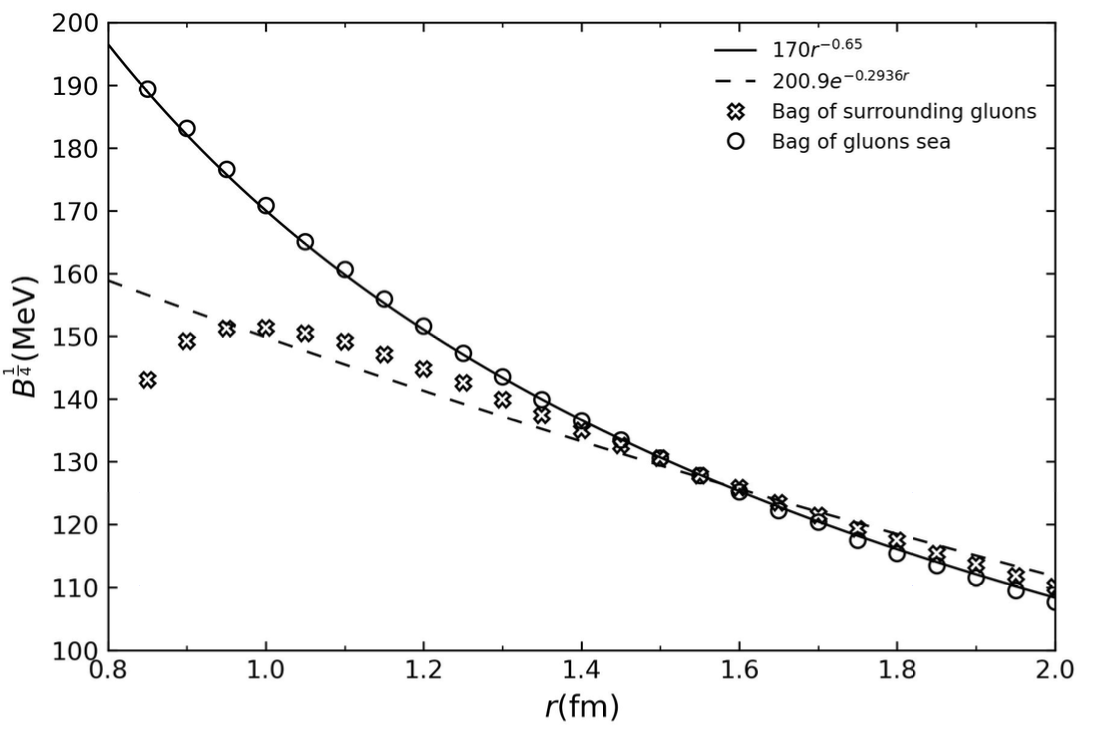
\includegraphics[width=0.58\textwidth]{./Images/B(R).png}

\caption[Presión de bolsa como función del radio del protón]{\emph{Ajuste realizado a una simulación numérica de la presión de bolsa dentro del protón como función del radio. Tenemos dos posibles escenarios: El primero (representado por las cruces) considera a los quarks rodeados por un mar de gluones, mientras que el segundo (círculos) considera a los quarks en un mar de gluones. []}}
\label{fig: B(r)}
\end{wrapfigure}

A partir del hecho de que la presión de bolsa depende del volumen de la misma, podemos pensar que la presión de bolsa cambiara con el radio (como se muestra en la figura \eqref{fig: B(r)}). Se pueden obtener los ajustes a ambos casos (el ajuste polinomial es el que mejor coeficiente de correlación obtiene para el caso de un mar de gluones), 

\begin{equation}\label{eq-B(r)-seagluons}
{B}^{1/4} = 0.17 \left[\frac{GeV}{fm}\right] {r}^{-0.65}
\end{equation}

o un ajuste exponencial para el segundo caso, gluones rodeando quarks, que obtiene, de entre varios otros ajustes (lineal, exponencial, logarítmico, polinomial) el mejor coeficiente de correlación

\begin{equation}\label{eq-B(r)-gluonssorrounding}
{B}^{1/4} = 0.201  {e}^{-0.293\left[\frac{1}{fm}\right]r} \left[{GeV}\right]
\end{equation}

Como una primera aproximación, usamos una presión de bolsa que es finita al centro del hadron y se desvanece a grandes distancias. Para este propósito, hemos determinado que una aproximación ajustable para la presión de bolsa es una exponencial de la forma \eqref{eq-B(r)-gluonssorrounding}, esta expresión, contiene el comportamiento que deseamos y esperamos para lo que sucede en el centro del hadrón, que en el centro la presión de la bolsa sea finita pero para grandes distancias se desvanezca.